%----------------------------------------------------------------------------
\appendix
%----------------------------------------------------------------------------
\chapter*{\fuggelek}\addcontentsline{toc}{chapter}{\fuggelek}
\setcounter{chapter}{\appendixnumber}
%\setcounter{equation}{0} % a fofejezet-szamlalo az angol ABC 6. betuje (F) lesz
\numberwithin{equation}{section}
\numberwithin{figure}{section}
\numberwithin{lstlisting}{section}
%\numberwithin{tabular}{section}
%TODO Függelék megadása - Programkód, adathalmazok githubon
%\( \faGit \faGit* \faGithub \faGitSquare \)
%----------------------------------------------------------------------------
\section{A megvalósított CUDA kódok elérése}
%----------------------------------------------------------------------------
Jelen dolgozat készítése során több CUDA keretrendszer segítségével több programot is írtam. Ezek forráskódját nyilvánosan elérhetővé tettem, a következő github linken elérhető a tesztadatokkal együtt: \textcolor{red}{LINK} 
\begin{figure}[!ht]
\centering
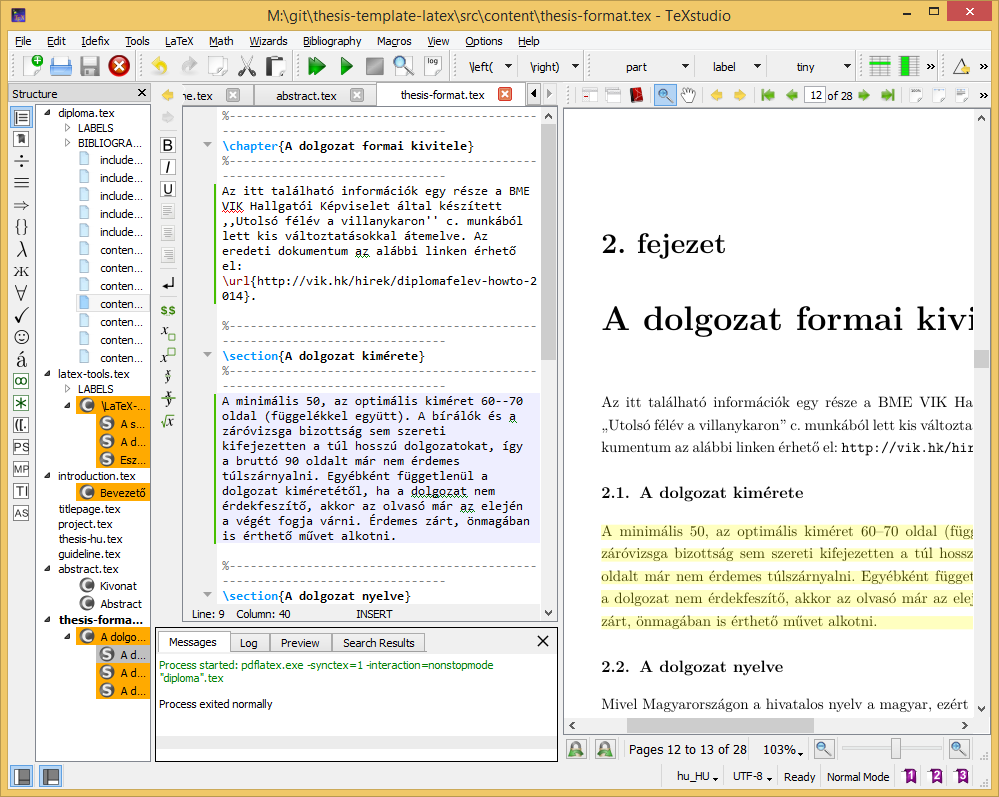
\includegraphics[width=150mm, keepaspectratio]{figures/TeXstudio.png}
\caption{A TeXstudio \LaTeX-szerkesztő.} 
\end{figure}


%----------------------------------------------------------------------------
\clearpage\section{A dolgozat során használt rövidítések}
%----------------------------------------------------------------------------

